% !TeX root = RJwrapper.tex
\title{corVis: An R Package for Visualising Associations and Conditional
Associations}
\author{by Amit Chinwan and Catherine Hurley}

\maketitle

\abstract{%
Correlation matrix displays are important tools to explore multivariate
datasets. These displays with other measures of association can
summarize interesting patterns to an analyst and assist them in framing
questions while performing exploratory data analysis. In this paper, we
present new visualisation techniques to visualise association between
all the variable pairs in a dataset in a single plot, which is something
existing displays lack. Also, we propse new methods to visualise
relationship among variable pairs using conditioning. We use different
layouts like matrix or linear for our displays. We use seriation in our
displays which helps in highlighting interesting patterns easily. The R
package \texttt{corVis} provides an implementation.
}

\hypertarget{section-1-introduction}{%
\section{Section 1: Introduction}\label{section-1-introduction}}

Correlation matrix display is a popular tool to visually explore
correlations among variables while performing Exploratory Data Analysis
(EDA) on a multivariate dataset. Popularized by
\citet{friendly2002corrgrams} as corrgram, these displays are produced
by first calculating the correlation among the variables and then
plotting these calculated values in a matrix display. With effective
ordering techniques, these displays quickly highlight variables which
are highly correlated and an analyst interested in building a predictive
model could use these displays to remove correlated variables and avoid
multicollinearity.

The correlation displays are generally used with one of the Pearson's,
Spearman's or Kendall's correlation coefficient and are therefore
limited to quantitative variables. An analyst can use one-hot encoding
of the qualitative variables in order to use these displays but will
need to deal with the high dimensions as a result of the encoding. In
addition to the dimensionality problem, it is not easy to assess the
overall correlation when using the one-hot encoding. The existing
methods to quickly explore association among qualitative variables in a
dataset include using proportions or counts with different graphical
displays like boxplots or barplots. Using association measures for
qualitative pairs similar to correlation for quantitative pairs will
help in summarizing the relationship, which then can be displayed like
the correlation displays.

Tukey and Tukey \citep{tukey1985computer} introduced scagnostics which
are measures for scatterplots. Along with scagnostics, they proposed a
scagnostics scatterplot matrix which is a visual display to explore and
compare these measures for all the variable pairs in a dataset. By
comparing multiple measures at once, the unusual variable pairs could be
identified and looked at in more detail. In a similar manner, a display
comparing association measures will help in finding interesting variable
pairs. Many association measures have been proposed to summarize
different types of relationships. The most commonly used measure is
Pearson's correlation coefficient which captures any linear trend
present between the variables. Other popular measures include Kendall's
or Spearman's rank correlation coefficient which are non-parametric
measures and looks for monotonic relationship. Distance correlation
\citep{szekely2007measuring} is an important measure useful in exploring
non-linear relationships. The information theory measure maximal
information coefficient (MIC) \citep{reshef2011detecting} is capable of
summarizing complex relationships. With effective displaying techniques,
the multiple measures of association provide a comparison tool that
assist an analyst to reveal structure present in the data.

Small multiples (or Trellis display) is a simple yet powerful approach
to compare partitions of data and understand multidimensional datasets
\citep{tufte1986thevisual}. The display is produced by splitting the
data into groups by a conditioning variable and then plotting the data
for each group. Such displays allow analysts to quickly infer about the
impact of the conditioning variable. A similar idea applied to displays
of association measures (correlation plot) will help uncover underlying
patterns in the data. One such pattern is Simpson's paradox which can be
detected by comparing Pearson's correlation for data at overall level
versus individual levels of the conditioning variable.

In this paper, we propose extensions of the correlation plot and new
visualizations which look at variables of mixed type, multiple
association measures and conditional associations. These displays are
implemented in the R package \CRANpkg{corVis}. The next section provides
a review of existing packages which deal with correlation displays and a
quick background on association measures and the packages used for
calculating them. Then we describe our approach to calculate the
association measures, followed by visualizations of associations and
conditional associations. We conclude with a summary and future work.

\hypertarget{section-2-background}{%
\section{Section 2: Background}\label{section-2-background}}

In this section we provide a brief review of existing packages used for
correlation displays and association measure calculation.

\hypertarget{section-2.1-literature-review-on-correlation-displays}{%
\subsection{Section 2.1: Literature Review on Correlation
Displays}\label{section-2.1-literature-review-on-correlation-displays}}

According to \citet{hills1969looking}, ``the first and sometimes only
impression gained by looking at a large correlation matrix is its
largeness''. To overcome this, \citet{murdoch1996graphical} proposed a
display for large correlation matrices which uses a matrix layout of
ellipses where the parameters of the ellipses are scaled to the
correlation values. \citet{friendly2002corrgrams} expanded on this idea
by rendering correlation values as shaded squares, bars, ellipses, or
circular `pac-man' symbols. The variables in the matrix displays were
optionally ordered using the angular ordering of the first two eigen
vectors of the correlation matrix. The ordering places highly-correlated
pairs of variables nearby, making it easier to quickly identify groups
of variables with high mutual correlation.

Nowadays, there are many R packages devoted to correlation
visualisation. Table \ref{tab:corrdisplay-packages} provides a summary,
listing the displays offered, and whether these extend to factor
variables or mixed numeric-factor pairs.

The R package \CRANpkg{corrplot} \citep{corrplot2021} provides an
implementation of the methods in \citet{friendly2002corrgrams}. The
package \CRANpkg{corrr} \citep{corrr2020} organises correlations as tidy
data, so leveraging the data manipulation and visualisation tools of the
\CRANpkg{tidyverse} \citep{tidyverse}. In addition to various matrix
displays, the package offers network displays where line-thickness
encodes correlation magnitude, with a filtering option to discard
low-correlation edges.

The package \CRANpkg{corrgrapher} \citep{corrgrapher} uses a network
plot for exploring correlations, where the nodes close to each other
have high correlation magnitude, edge thickness encodes the absolute
correlation value and edge color indicates the sign of correlation. The
package also handles mixed type variables by using association measures
obtained as transformations of \(p\)-values obtained from Pearson's
correlation test in the case of two numeric variables, Kruskal's test
for numerical and factor variables, and a chi-squared test for two
categorical variables.

The package \CRANpkg{linkspotter} \citep{linkspotter} offers a variety
of association measures (distance correlation, MIC, maximum normalized
mutual information) in addition to correlation, where the measure used
depends on whether the variables are both numerical, categorical or
mixed. The results are visualized in a network plot, which may be
packaged into an interactive shiny application.

Our own package \CRANpkg{corVis} offers a variety of displays, and has
new features not available elsewhere, in particular simultaneous display
of multiple association measures, and association displays stratified by
levels of a grouping variable. This will be described in the following
sections.

There have been other extensions to correlation displays which are
useful when dealing with high dimensional datasets.
\citet{hills1969looking} proposed a QQ plot of the \(z\)-transform of
the entries of the correlation matrix to discover correlation
coefficients too large to come from a normal distribution with mean
zero. \citet{buja2016visualization} proposed Association Navigator which
is an interactive visualization tool for large correlation matrices with
upto 2000 variables. The R package \CRANpkg{scorrplot} \citep{scorr}
produces an interactive scatterplot for exploring pairwise correlations
in a large dataset by projecting variables as points and encoding the
correlations as space between these points. The package provides a
functionality to update variable of interest which creates tour of the
correlation space between different projections of the data.

The R package \CRANpkg{correlationfunnel} offers a novel display which
assists in feature selection in a setting with a single response and
many predictor variables. All numeric variables including the response
are binned. All (now categorical) variables in the resulting dataset are
one-hot encoded and Pearson's correlation calculated with the response
categories. The correlations are visualised in a dot-plot display, where
predictors are ordered by maximum correlation magnitude. Correlations
between one-hot encoded variables are challenging to interpret,
especially as the number of levels increase. In corVis we offer a
similar dot-plot display, but showing multiple correlation or
association measures, or alternatively measures stratified by a grouping
variable.

\begin{Schunk}
\begin{table}

\caption{\label{tab:corrdisplay-packages}List of the R packages dealing with correlation or correlation displays with information on whether the plots display multiple measures, conditional display of measures and mixed variables in a single plot}
\centering
\begin{tabular}[t]{lll}
\toprule
Package & Display & MixedVariables\\
\midrule
corrplot & heatmap & \\
corrr & heatmap/network & \\
corrgrapher & network & \\
linkspotter & network & Yes\\
correlation & heatmap/network & \\
\addlinespace
corVis & heatmap/matrix/linear & Yes\\
\bottomrule
\end{tabular}
\end{table}

\end{Schunk}

\hypertarget{section-2.2-literature-review-on-association-measures}{%
\subsection{Section 2.2: Literature Review on Association
Measures}\label{section-2.2-literature-review-on-association-measures}}

An association measure is defined as a numerical summary quantifying the
relationship between two or more variables. The measure is called
symmetric if its value is invariant to the choice of independent or
dependent variable during the calculation. For example, Pearson's
correlation coefficient summarizes the strength and direction of the
linear relationship present between two numeric variables in the range
\([-1,1]\) and is symmetric. Kendall's or Spearman's rank correlation
coefficient are other popular measures which assess monotonic
relationship among two numeric variables in interval \([-1,1]\) and are
symmetric measures.

Pearson's correlation is the most popular association measure because of
its easier calculation and interpretability but its limitations such as
influence of outliers on its value and measuring only linear
dependencies makes it a less useful measure of association overall. The
recent measures such as distance correlation
\citep{szekely2007measuring} and MIC \citep{reshef2011detecting}
overcome these limitations and are more suitable for datasets with both
linear and non-linear patterns.

\begin{Schunk}
\begin{figure}

{\centering 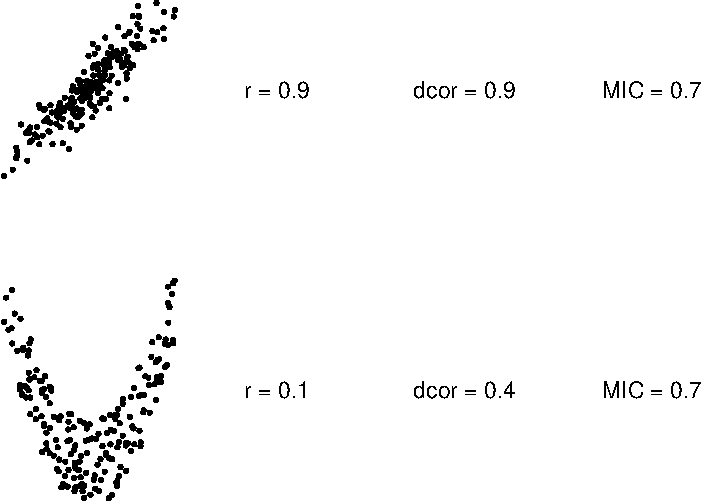
\includegraphics{rj_paper_files/figure-latex/motivation-patterns-1} 

}

\caption[Multiple association measures for simulated linear and non-linear pattern]{Multiple association measures for simulated linear and non-linear pattern. The first row of the plot shows a linear pattern, the value of Pearson's correlation, distance correlation and MIC. The second row of the plot shows a non-linear pattern along with the values for association measures. All three association measures show a high value for the linear relationship and hence are useful for linear patterns. For non-linear pattern, distance correlation and MIC are more suitable measures than Pearson's correlation.}\label{fig:motivation-patterns}
\end{figure}
\end{Schunk}

Figure \ref{fig:motivation-patterns} shows a plot of simulated linear
and non-linear patterns. The first row shows a linear relationship along
with the value for measures such as Pearson's correlation, distance
correlation and maximal information coefficient respectively for the
pattern. In a similar manner, the second row shows a quadratic
relationship and its values for Pearson's correlation, distance
correlation and maximal information coefficient respectively.\\
It is clearly evident from Figure \ref{fig:motivation-patterns} that all
the three measures summarizes the pattern with linear relationship quite
well. For the non-linear pattern, distance correlation and MIC are
better in detecting underlying relationship than Pearson's correlation.
This suggests that association measures such as distance correlation,
MIC and other measures should be used along with Pearson's correlation
for exploring relationships among variables in the datasets where there
is no prior knowledge about the possible patterns in the data.

The distance correlation coefficient \citep{szekely2007measuring} is an
association measure which looks for any relationship among two numeric
variables using the distances between observations of these variables
and summarizes the relationship in \([0,1]\). The distance correlation
is \(0\) only when the variables are independent and is a symmetric
measure.

The maximal information coefficient (MIC) \citep{reshef2011detecting} is
an information theory measure which uses mutual information among the
two variables for its calculation. The main idea is to find a grid out
of possible grids on a scatterplot of two numeric variables, in order to
discretize the variables, which maximises the mutual information for the
two variables. A normalisation technique is used to make the mutual
information from different grids comparable. Referred as `a correlation
of 21st century' {[}speed2011correlation{]}, MIC is capable of
summarizing different types of relationships, not just linear or
monotonous, between numeric variables and is in range \([0,1]\).
\citet{reshef2011detecting} used MIC and other related statistics to
explore pairwise relationships in large data sets such as major-league
baseball, gene expression, global health, and the human gut microbiota.

In addition to association measures for numeric variables, association
measures for ordinal, nominal and mixed variable pairs are useful in
exploring a multivariate dataset. We now give an overview of available
association measures for other variable types.

\citet{agresti2010analysis} provides an overview of the association
measures which are used for exploring association between ordinal
variables. Kendall's tau-b \citep{kendall1945treatment} is an
association measure useful in summarizing the relationship between two
ordinal variables in the range \([-1,1]\). It is a relatively stable
measure than Goodman and Kruskal's gamma with respect to the changes in
categories of any variable i.e.~if two categories are merged to make a
single category. The polychoric correlation \citep{olsson1979maximum}
measures the correlation between two ordinal variables by assuming two
normally distributed latent variables for a contingency table of two
ordinal variables and summarizes the association in \([-1,1]\).

The association measures for the case of nominal pair of variables
should be invariant to the order in which the categories appear.
Pearson's contingency coefficient uses the \({\chi}^2\) value from the
Pearson's \({\chi}^2\) test for independence and is a useful measure to
summarize the association between two nominal variables in \([0,1]\).
Another measure for nominal variable pair is the Uncertainty coefficient
\citep{theil1970estimation} measuring the proportion of uncertainty in
one variable which is explained by the other variable.

\hypertarget{section-3-introducing-corvis}{%
\section{Section 3: Introducing
corVis}\label{section-3-introducing-corvis}}

\CRANpkg{corVis} is an R package which calculates measures of
association for every variable pair in a dataset and provides
visualizations for displaying associations. Most of the existing
correlation displays are limited to numeric pairs of variables. This
package extends these displays to every variable pair. The main goal of
our work is to propose displays for multiple association measures and
conditional associations display which are useful for uncovering
interesting patterns in the data. This will help in identifying variable
pairs which shows a type of relationship or pattern in a dataset with
large number of variables.

\begin{Schunk}
\begin{figure}

{\centering 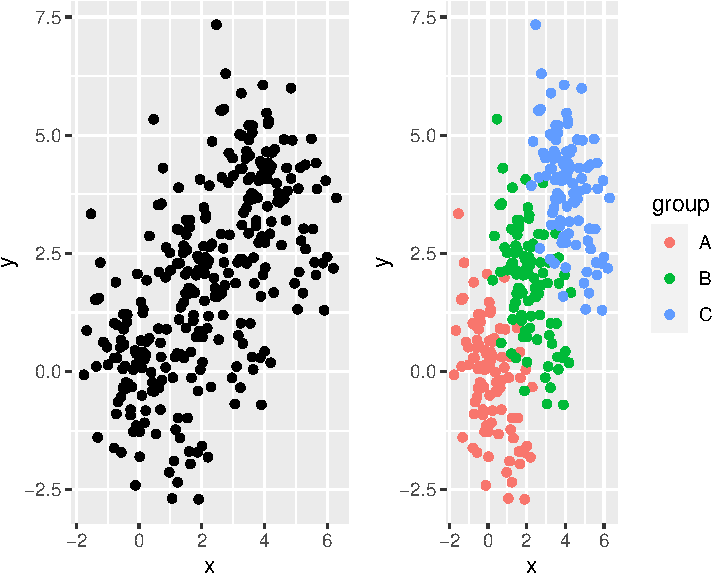
\includegraphics{rj_paper_files/figure-latex/motivation2-1} 

}

\caption[An example plot showing importance of conditional displays]{An example plot showing importance of conditional displays}\label{fig:motivation2}
\end{figure}
\end{Schunk}

Consider Figure \ref{fig:motivation2} for the motivation behind
conditional association displays. The plot on the left shows a positive
linear association between \texttt{y} and \texttt{x} and has a positive
Pearson's correlation of value 0.603. The plot on the right shows the
disaggregated data by the \texttt{group} variable and it is clearly
evident that for each group there is a negative linear relationship
between \texttt{y} and \texttt{x}. This is an example of Simpson's
paradox and is one of the patterns which are discoverable when
conditional association displays are used.

While designing these displays we considered matrix and linear layouts.
A matrix layout simplifies the effort in finding variables, and
different measures may be displayed on the upper and lower diagonal.
Linear layouts are more space-efficient than matrix plots, but looking
for variables or variable pairs is more challenging.

Table \ref{tab:function-corVis} provides a list of the functions
available in the package which are useful for calculating association
measures among variable pairs and visualising these associations using
novel displays. Section 4 provides a detailed description on functions
used for calcuating association measures in the package. Section 5
illustrates the use of visualising functions in table
\ref{tab:function-corVis} for displaying pairwise association and
conditional association.

\begin{Schunk}
\begin{table}

\caption{\label{tab:function-corVis}List of functions in corVis package}
\centering
\begin{tabular}[t]{>{}l|l|l}
\hline
Function & Usage & Description\\
\hline
\textbf{calc\_assoc} & Calculation & Calculates association measures\\
\hline
\textbf{association\_heatmap} & Visualization & Conventional correlation matrix plot\\
\hline
\textbf{pairwise\_2d\_plot} & Visualization & Conditional and multiple measures matrix plot\\
\hline
\textbf{pairwise\_1d\_plot} & Visualization & Conditional and multiple measures linear plot\\
\hline
\end{tabular}
\end{table}

\end{Schunk}

\hypertarget{section-4-corvis-calculating-association}{%
\section{Section 4: corVis: Calculating
Association}\label{section-4-corvis-calculating-association}}

This section describes the calculation of association measures in our
package \CRANpkg{corVis}. The package provides a standard interface for
calculating a collection of various measures of association which
quantifies the relationship between two variables. The association
measures available in the package are not limited to numeric variables
and are used with nominal, ordinal and mixed variable pairs as well. The
package also provides a functionality for handling missing value or
\texttt{NA} while calculating the association measures.

Table \ref{tab:association-measures} lists different functions provided
in the package to calculate varoius measures of association. The
\texttt{Function} column represents the function name used to calculate
measure(s) of associations in this package. The \texttt{typeX} and
\texttt{typeY} columns provide the information on types of variables
which can be used with the corresponding functions. The \texttt{X} or
\texttt{Y} variable is one of the numeric, nominal, ordinal or any type.
The \texttt{from} column corresponds to the package functions used to
calculate the association measures by the function under
\texttt{Function}. The \texttt{symmetric} column represents if the
measure is symmetric i.e.~if the value of measure is same regardless of
the order of variables. The last column provides the range of values for
these measures. The function \texttt{tbl\_easy} calculates association
measures available in the R package \CRANpkg{correlation} and is
suitable for different variable types. The functions in Table
\ref{tab:association-measures} with \texttt{corVis} entries under
\texttt{from} column calculate the association measures which have been
implemented in this package.

For numeric pairs of variables, this package provides a range of
association measures. The popular correlation coefficients like
Pearson's or Spearman's or Kendall's are calculated using
\texttt{tbl\_cor} function. The measures such as distance correlation or
MIC are calculated using \texttt{tbl\_dcor} or \texttt{tbl\_mine}
respectively. The association measures available in the package for the
ordinal pairs of variables are polychoric correlation and Kendall's
coefficients which are calculated using \texttt{tbl\_polycor} or
\texttt{tbl\_tau} respectively. For nominal pairs of variables, the
functions like \texttt{tbl\_gkTau}, \texttt{tbl\_gkGamma},
\texttt{tbl\_uncertainty}, \texttt{tbl\_chi}, \texttt{tbl\_cancor} are
used for exploring association among the variables.

The function \texttt{tbl\_cancor} calculates a measure of association
based on canonical correlations for mixed pairs of variables. Nominal
variables are converted into sets of dummy variables, which are then
assigned scored to find the maximal correlation. For two numeric
variables this measure is identical to absolute correlation, for two
factors the correlation is identical to that obtained from
correspondence analysis.

The functions listed in \ref{tab:association-measures} for calculating
association measures provide a functionality for handling missing value
or \texttt{NA} in the dataset. Each of these functions either have a
\texttt{handle.na} argument or have package functions which
automatically uses pairwise complete observations for taking care of
missing values present in the data.

\begin{Schunk}
\begin{table}

\caption{\label{tab:association-measures}List of the functions available in the package for calculating different association measures along with the packages used for calculation.}
\centering
\begin{tabular}[t]{llllll}
\toprule
Function & X & Y & from & symmetric & range\\
\midrule
tbl\_cor & numerical & numerical & stats::cor & Y & {}[-1,1]\\
tbl\_dcor & numerical & numerical & energy::dcor2d & Y & {}[0,1]\\
tbl\_mine & numerical & numerical & minerva::mine & Y & {}[0,1]\\
tbl\_polycor & ordinal & ordinal & polycor::polychor & Y & {}[-1,1]\\
tbl\_tau & ordinal & ordinal & DescTools::KendalTauA,B,C,W & Y & {}[-1,1]\\
\addlinespace
tbl\_gkGamma & ordinal & ordinal & DescTools::GoodmanKruskalGamma & Y & {}[0,1]\\
tbl\_gkTau & nominal & nominal & DescTools::GoodmanKruskalTau & N & {}[0,1]\\
tbl\_uncertainty & nominal & nominal & DescTools::UncertCoef & Y & {}[0,1]\\
tbl\_chi & nominal & nominal & DescTools::ContCoef & Y & {}[0,1]\\
tbl\_cancor & nominal/numerical & nominal/numerical & corVis & Y & {}[0,1]\\
\addlinespace
tbl\_nmi & any & any & corVis & Y & {}[0,1]\\
tbl\_easy & any & any & correlation::correlation & Y & {}[-1,1]\\
\bottomrule
\end{tabular}
\end{table}

\end{Schunk}

\hypertarget{calculating-association-for-a-single-type-of-variable-pairs}{%
\subsection{Calculating association for a single type of variable
pairs}\label{calculating-association-for-a-single-type-of-variable-pairs}}

We have a function which creates a tibble structure for the variable
pairs in a dataset along with calculated association measure. The
package contains various functions (shown in Table
\ref{tab:association-measures}) for different association measures in
the form \texttt{tbl\_*} to calculate them. For example, in order to
calculate distance correlation for numeric pair of variables in a
dataset, the function \texttt{tbl\_dcor} is used.

\begin{Schunk}
\begin{Sinput}
ckd <- RWeka::read.arff("../data/chronic_kidney_disease.arff")
df <- ckd
#df$al <- as.ordered(df$al)
#df$su <- as.ordered(df$su)

distance <- tbl_dcor(df)
distance
\end{Sinput}
\begin{Soutput}
#> # A tibble: 55 x 4
#>    x     y     measure measure_type
#>    <chr> <chr>   <dbl> <chr>       
#>  1 bp    age     0.189 dcor        
#>  2 bgr   age     0.303 dcor        
#>  3 bu    age     0.249 dcor        
#>  4 sc    age     0.242 dcor        
#>  5 sod   age     0.154 dcor        
#>  6 pot   age     0.119 dcor        
#>  7 hemo  age     0.254 dcor        
#>  8 pcv   age     0.296 dcor        
#>  9 wbcc  age     0.173 dcor        
#> 10 rbcc  age     0.307 dcor        
#> # ... with 45 more rows
\end{Soutput}
\end{Schunk}

The tibble output for the functions mentioned in Table
\ref{tab:association-measures} has the following structure:

\begin{itemize}
\tightlist
\item
  \texttt{x} and \texttt{y} representing a pair of variables
\item
  \texttt{measure} representing the calculated value for association
  measure
\item
  \texttt{measure\_type} representing the association measure calculated
  for \texttt{x} and \texttt{y} pair.
\end{itemize}

\hypertarget{calculating-association-measures-for-whole-dataset}{%
\subsection{Calculating association measures for whole
dataset}\label{calculating-association-measures-for-whole-dataset}}

\texttt{calc\_assoc} is used to calculate association measures for all
the variable pairs in the dataset at once in a tibble structure. The
variable pairs in the output are unique pairs and a subset of all the
pairs of variables in a dataset where \texttt{x} \(\neq\) \texttt{y}.
Because of the tidy structure of the output, the data manipulation and
visualisation tools of \CRANpkg{tidyverse} \citep{tidyverse} are
applicable to and are useful for further exploration of pairwise
associations. In addition to tibble structure, the output also has
\texttt{pairwise} and \texttt{data.frame} class which are important
class attributes for producing visual summaries in this package.

The function \texttt{calc\_assoc} has a \texttt{types} argument which is
basically a tibble of the association measure to be calculated for
different variable pairs. The default tibble of measures is
\texttt{default\_assoc()} which calculates Pearson's correlation if both
the variables are numeric, Kendall's tau-b if both the variables are
ordinal, canonical correlation if one is factor and other is numeric and
canonical correlation for the rest of the variable pairs.

\begin{Schunk}
\begin{Sinput}
default_measures <- default_assoc()
default_measures
\end{Sinput}
\begin{Soutput}
#> # A tibble: 4 x 4
#>   funName    typeX   typeY   argList
#>   <chr>      <chr>   <chr>   <list> 
#> 1 tbl_cor    numeric numeric <NULL> 
#> 2 tbl_tau    ordered ordered <NULL> 
#> 3 tbl_cancor factor  numeric <NULL> 
#> 4 tbl_cancor other   other   <NULL>
\end{Soutput}
\begin{Sinput}
ckd_assoc <- calc_assoc(df,types = default_assoc())
ckd_assoc
\end{Sinput}
\begin{Soutput}
#> # A tibble: 300 x 4
#>    x     y     measure measure_type
#>    <chr> <chr>   <dbl> <chr>       
#>  1 bp    age    0.159  pearson     
#>  2 sg    age    0.199  cancor      
#>  3 al    age    0.235  cancor      
#>  4 su    age    0.287  cancor      
#>  5 rbc   age    0.0800 cancor      
#>  6 pc    age    0.151  cancor      
#>  7 pcc   age    0.158  cancor      
#>  8 ba    age    0.0422 cancor      
#>  9 bgr   age    0.245  pearson     
#> 10 bu    age    0.197  pearson     
#> # ... with 290 more rows
\end{Soutput}
\begin{Sinput}
class(ckd_assoc)
\end{Sinput}
\begin{Soutput}
#> [1] "pairwise"   "tbl_df"     "tbl"        "data.frame"
\end{Soutput}
\end{Schunk}

The default tibble of measures is updated using the
\texttt{update\_assoc} function which has arguments for updating the
\texttt{tbl\_*} functions to calculate association measures depending on
the type variable pair in the dataset and a method for \texttt{tbl\_*}
functions which calculates more than one measure. The
\texttt{update\_assoc} function has an argument \texttt{default} which
has the \texttt{default\_assoc()} tibble as its default value and is
useful when \texttt{tbl\_*} functions need to be updated for a few types
of variable pairs.

\begin{Schunk}
\begin{Sinput}
updated_assoc <- update_assoc(default=default_assoc(),
                              num_pair = "tbl_cor",
                              num_pair_argList = "spearman",
                              mixed_pair = "tbl_cancor",
                              other_pair = "tbl_nmi")
updated_assoc
\end{Sinput}
\begin{Soutput}
#> # A tibble: 4 x 4
#>   funName    typeX   typeY   argList  
#>   <chr>      <chr>   <chr>   <list>   
#> 1 tbl_cor    numeric numeric <chr [1]>
#> 2 tbl_tau    ordered ordered <NULL>   
#> 3 tbl_cancor factor  numeric <NULL>   
#> 4 tbl_nmi    other   other   <NULL>
\end{Soutput}
\end{Schunk}

\texttt{calc\_assoc} also has a \texttt{handle.na} argument for handling
the \texttt{NA} or missing values which is fed into the \texttt{tbl\_*}
functions used with the \texttt{types} argument for different types of
variable pairs. The default value is set to \texttt{TRUE} for using
pairwise complete observations for calculating a measure of association
between two variables.

If a user is interested in calculating multiple association measures for
a type of variable pair, it can be done by using the
\texttt{calc\_assoc} and \texttt{update\_assoc} together for calculating
different association measures and then merging the output tibbles.

\begin{Schunk}
\begin{Sinput}
updated_ckd_assoc <- calc_assoc(df, types = updated_assoc)
updated_ckd_assoc
\end{Sinput}
\begin{Soutput}
#> # A tibble: 300 x 4
#>    x     y     measure measure_type
#>    <chr> <chr>   <dbl> <chr>       
#>  1 bp    age    0.123  spearman    
#>  2 sg    age    0.199  cancor      
#>  3 al    age    0.235  cancor      
#>  4 su    age    0.287  cancor      
#>  5 rbc   age    0.0800 cancor      
#>  6 pc    age    0.151  cancor      
#>  7 pcc   age    0.158  cancor      
#>  8 ba    age    0.0422 cancor      
#>  9 bgr   age    0.299  spearman    
#> 10 bu    age    0.309  spearman    
#> # ... with 290 more rows
\end{Soutput}
\end{Schunk}

\hypertarget{calculating-conditional-association}{%
\subsection{Calculating conditional
association}\label{calculating-conditional-association}}

\texttt{calc\_assoc} is also used to calculate association measures for
all the variable pairs at different levels of a categorical variable.
This helps in exploring the conditional associations and find out the
differences between the groups of the conditioning variable. The
function has a \texttt{by} argument which is used as the grouping
variable and needs to be categorical.

\begin{Schunk}
\begin{Sinput}
ckd_assoc_by <- calc_assoc_by(df,by = "htn")
ckd_assoc_by
\end{Sinput}
\begin{Soutput}
#> # A tibble: 1,104 x 5
#>    x     y      measure measure_type by   
#>    <chr> <chr>    <dbl> <chr>        <fct>
#>  1 bp    age   -0.112   pearson      yes  
#>  2 sg    age    0.0240  cancor       yes  
#>  3 al    age    0.130   cancor       yes  
#>  4 su    age    0.219   cancor       yes  
#>  5 rbc   age    0.115   cancor       yes  
#>  6 pc    age    0.101   cancor       yes  
#>  7 pcc   age    0.0609  cancor       yes  
#>  8 ba    age    0.00562 cancor       yes  
#>  9 bgr   age    0.0303  pearson      yes  
#> 10 bu    age   -0.135   pearson      yes  
#> # ... with 1,094 more rows
\end{Soutput}
\end{Schunk}

By default, the function \texttt{calc\_assoc} calculates the association
measures for all the variable pairs at different levels of the grouping
variable and the pairwise association measures for the ungrouped data
(\texttt{overall}) when used with the \texttt{by} argument. This
behavior can be changed by setting \texttt{include.overall} argument to
\texttt{FALSE}.

\begin{Schunk}
\begin{Sinput}
ckd_assoc_by <- calc_assoc_by(df,by = "htn",include.overall = FALSE)
ckd_assoc_by
\end{Sinput}
\begin{Soutput}
#> # A tibble: 828 x 5
#>    x     y      measure measure_type by   
#>    <chr> <chr>    <dbl> <chr>        <fct>
#>  1 bp    age   -0.112   pearson      yes  
#>  2 sg    age    0.0240  cancor       yes  
#>  3 al    age    0.130   cancor       yes  
#>  4 su    age    0.219   cancor       yes  
#>  5 rbc   age    0.115   cancor       yes  
#>  6 pc    age    0.101   cancor       yes  
#>  7 pcc   age    0.0609  cancor       yes  
#>  8 ba    age    0.00562 cancor       yes  
#>  9 bgr   age    0.0303  pearson      yes  
#> 10 bu    age   -0.135   pearson      yes  
#> # ... with 818 more rows
\end{Soutput}
\end{Schunk}

The tibble output in the conditional setting has a similar structure as
\texttt{calc\_assoc} used with no \texttt{by} argument. When used with
the \texttt{by} argument, an additional \texttt{by} column representing
the levels of the categorical variable is added in the tibble output.
The \texttt{x} and \texttt{y} variables in the output are repeated for
every level of \texttt{by} variable. In order to have multiple
\texttt{by} variables, the function \texttt{calc\_assoc} is used
multiple times with a different \texttt{by} variable each time and then
the multiple outputs are binded row wise. For calculating multiple
measures for a specific variable type, one can use
\texttt{update\_assoc} with \texttt{calc\_assoc} and then can merge
these multiple tibble outputs.

\hypertarget{section-5-corvis-visualising-association}{%
\section{Section 5: corVis: Visualising
Association}\label{section-5-corvis-visualising-association}}

This section provides a detailed description of the novel visualisation
techniques proposed in the package \CRANpkg{corVis}. These methods
display association and conditional association for every variable pair
in a dataset in a single plot and show multiple bivariate measures of
association simultaneously.

We use chronic kidney dataset providing information on early stage of
Chronic Kidney Disease(CKD) patients from the \citep{Dua:2019} to
provide illustrative examples. Table \ref{tab:ckd} provides a brief
description of set of variables from this dataset used for analysis.

\begin{Schunk}
\begin{table}

\caption{\label{tab:ckd}Variable description of the chronic kidney dataset along with the types of variables}
\centering
\begin{tabular}[t]{lll}
\toprule
Variable & Description & VariableType\\
\midrule
bgr & Blood Glucose Random in mgs/dl & numerical\\
bu & Blood Urea mgs/dl & numerical\\
rbcc & Red Blood Cell Count in millions/cmm & numerical\\
pcv & Packed  Cell Volume & numerical\\
sod & Sodium in mEq/L & numerical\\
\addlinespace
sc & Serum Creatinine in mgs/dl & numerical\\
al & Albumin (0,1,2,3,4,5) & ordinal\\
su & Sugar (0,1,2,3,4,5) & ordinal\\
htn & Hypertension (yes,no) & nominal\\
dm & Diabetes Mellitus (yes,no) & nominal\\
\addlinespace
cad & Coronary Artery Disease (yes,no) & nominal\\
\bottomrule
\end{tabular}
\end{table}

\end{Schunk}

\hypertarget{association-matrix-plot}{%
\subsection{Association Matrix plot}\label{association-matrix-plot}}

The function \texttt{association\_heatmap} is used to display a matrix
layout with association for variable pairs in the dataset. The display
is similar to existing correlation matrix plots but with every variable
pair in the dataset. This function \texttt{association\_heatmap} takes
the calculated measures of association by \texttt{calc\_assoc} function
as input and outputs a matrix display by rendering the magnitude of
association measures with a color. The function has \texttt{lassoc} and
\texttt{uassoc} arguments for a tibble of association measures for the
lower triangle and the upper triangle of the matrix display
respectively. The \texttt{uassoc} argument is \texttt{NULL} by default
and uses the same tibble input as used by \texttt{lassoc} if not
changed. The argument \texttt{var\_order} is used for ordering or
seriating the matrix display such that highly-associated variables are
placed nearby and are easier to identify. We use average linkage
hierarchical clustering method as the default method for ordering the
variables. The function also has a \texttt{limits} argument specifying
the limit of the color scale.

Figure \ref{fig:assoc-heatmap} shows an example of the association
matrix display for every variable pair in the chronic kidney disease
dataset. The cells along the diagonal of the matrix display show the
variables present in the dataset. Every off diagonal cell is colored
using a divergent color scale with limits \([-1,1]\) representing the
value of association measure between two variables. The plot shows
Pearson's correlation for the numeric pair of variables and canonical
correlation for mixed and nominal variable pairs.

\begin{Schunk}
\begin{Sinput}
ckd <- RWeka::read.arff("../data/chronic_kidney_disease.arff")

vars <- c("bgr","bu","rbcc","pcv","sod","sc","al","su","htn","dm","cad")
df <- ckd[,vars]
#df$al <- as.ordered(df$al)
#df$su <- as.ordered(df$su)

assoc <- calc_assoc(df)
association_heatmap(assoc)
\end{Sinput}
\begin{figure}

{\centering 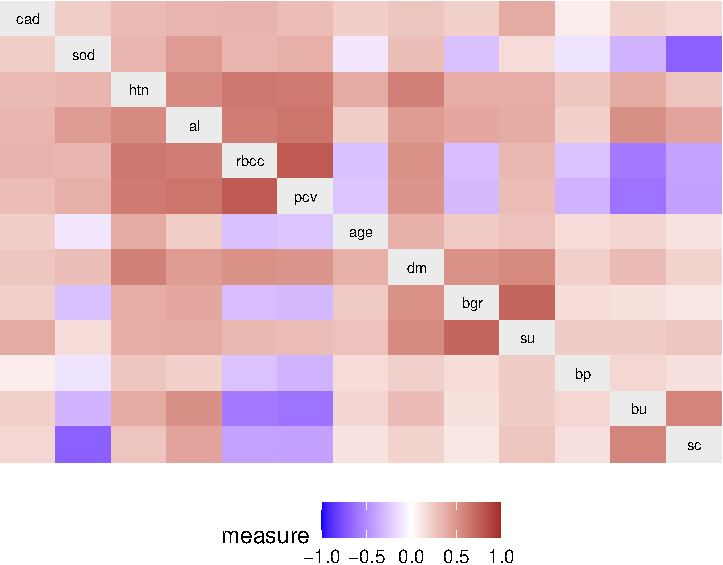
\includegraphics{rj_paper_files/figure-latex/assoc-heatmap-1} 

}

\caption[Association matrix display for kidney data showing Pearson's correlation for numeric variable pairs, canonical correlation for mixed variable pairs and categorical variable pairs]{Association matrix display for kidney data showing Pearson's correlation for numeric variable pairs, canonical correlation for mixed variable pairs and categorical variable pairs.}\label{fig:assoc-heatmap}
\end{figure}
\end{Schunk}

For numeric pairs, Figure \ref{fig:assoc-heatmap} shows a high positive
Pearson's correlation among \texttt{rbcc} and \texttt{pcv} and a high
negative Pearson's correlation between \texttt{sc} and \texttt{sod}.
Figure \ref{fig:numeric-pairs} shows scatterplot for these two pairs of
variables and is evident that these pairs seems to be linearly
associated.

\begin{Schunk}
\begin{figure}

{\centering 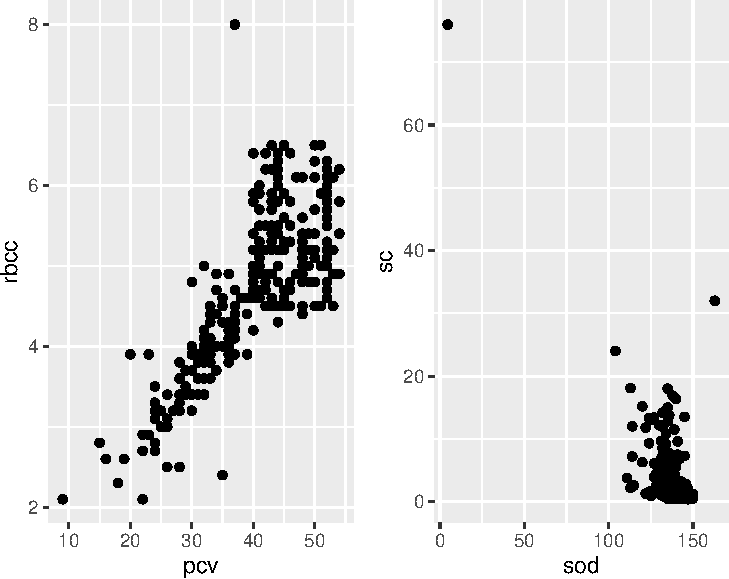
\includegraphics{rj_paper_files/figure-latex/numeric-pairs-1} 

}

\caption[Scatterplot for variables rbcc and pcv, and, sc and sod showing a high positive and negative Pearson's correlation respectively]{Scatterplot for variables rbcc and pcv, and, sc and sod showing a high positive and negative Pearson's correlation respectively.}\label{fig:numeric-pairs}
\end{figure}
\end{Schunk}

Figure \ref{fig:assoc-heatmap} shows a high canonical correlation
between \texttt{bgr} and \texttt{su}, \texttt{rbcc} and \texttt{htn},
and, \texttt{pcv} and \texttt{al} which are mixed variable pairs in the
dataset. These variable pairs are further looked into using boxplots.
Figure \ref{fig:mixed-pairs} shows boxplot for these variable pairs and
is evident there is an association among these variable pairs.

\begin{Schunk}
\begin{figure}

{\centering 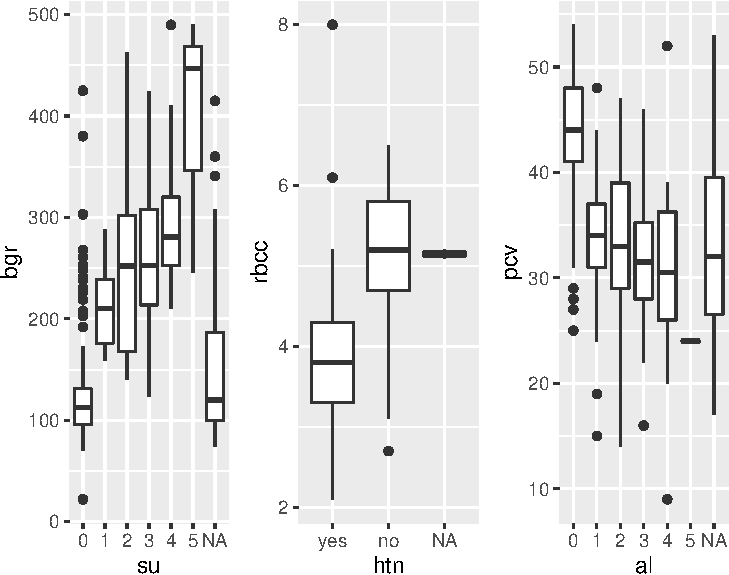
\includegraphics{rj_paper_files/figure-latex/mixed-pairs-1} 

}

\caption[Boxplot for variables bgr and su, htn and rbcc, and, al and pcv showing a high canonical correlation ]{Boxplot for variables bgr and su, htn and rbcc, and, al and pcv showing a high canonical correlation . }\label{fig:mixed-pairs}
\end{figure}
\end{Schunk}

For nominal variable pairs, Figure \ref{fig:assoc-heatmap} shows a high
canonical correlation among \texttt{htn} and \texttt{al}, \texttt{htn}
and \texttt{dm}, and, \texttt{dm} and \texttt{su}. These pairs of
variables can be further looked at by plotting proportional bar charts.

\hypertarget{multiple-association-measures-plot}{%
\subsection{Multiple Association Measures
Plot}\label{multiple-association-measures-plot}}

The function \texttt{pairwise\_1d\_compare} is used to display a linear
layout for comparing multiple association measures calculated for
variable pairs in the dataset. \texttt{pairwise\_1d\_compare} the
calculated association measures as input and outputs a heatmap display
by plotting all the variable pairs in the dataset on the Y-axis and the
association measures on the X-axis and encoding the magnitude of
association measures with a color.

The \texttt{assoc} argument of the function
\texttt{pairwise\_1d\_compare} represents a tibble of calculated
multiple association measures. These measures are calculated using
\texttt{tbl\_*} or \texttt{calc\_assoc} functions and are binded row
wise to create a tibble structure with multiple measures. The function
also has a \texttt{var\_order} argument which is set to
\texttt{max\_diff} by default and orders the variable pairs on the basis
of maximum difference among the magnitude of measures.

Figure \ref{fig:compare-linear} shows a linear layout comparing multiple
association measures for all the variable pairs in the chronic kidney
data. The plot shows that the variable pair sc and sod have a magnitude
for Pearson's correlation and a magnitude for Spearman's rank
correlation suggesting that the relationship among these variables might
not be linear and should be looked at in more detail. For variable pairs
sc and rbcc, and, sc and pcv, the Spearman's rank correlation has a high
magnitude indicating a presence of monotonic relationship for these
variable pairs.

\begin{Schunk}
\begin{Sinput}
pearson <- tbl_cor(df,method = "pearson")
spearman <- tbl_cor(df, method = "spearman")
distance <- tbl_dcor(df)
mic <- tbl_mine(df)
cancor <- tbl_cancor(df)

assoc <- rbind(pearson, spearman, distance, mic, cancor)

pairwise_1d_compare(assoc)
\end{Sinput}
\begin{figure}

{\centering 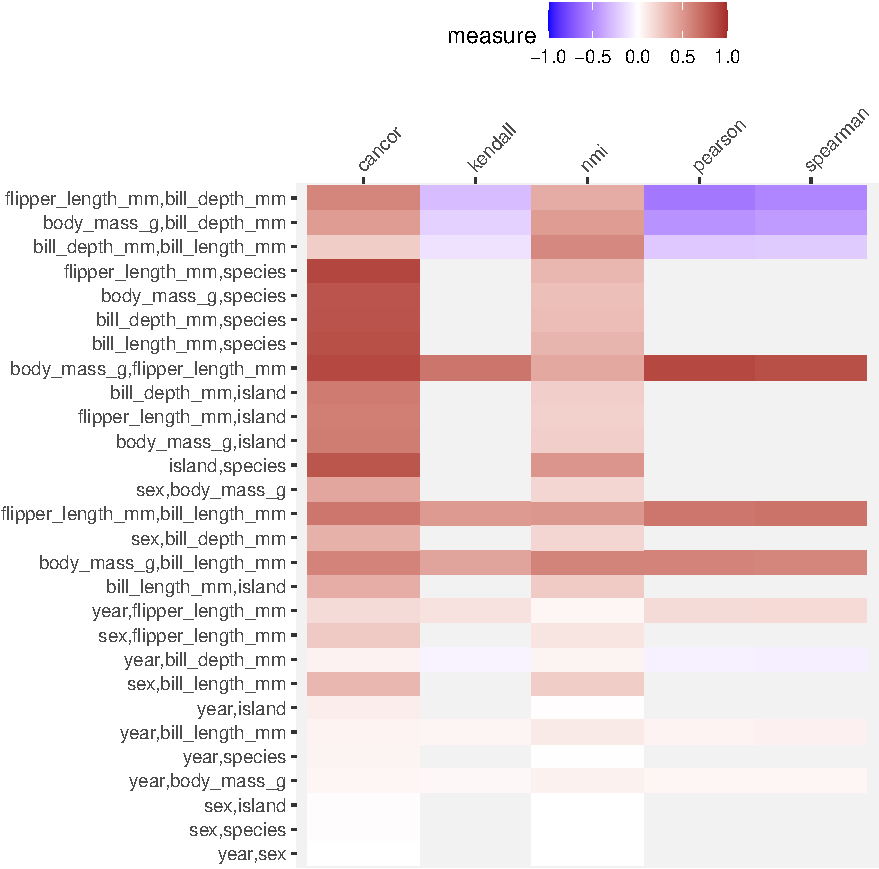
\includegraphics{rj_paper_files/figure-latex/compare-linear-1} 

}

\caption[Comparing multiple association measures using a linear layout]{Comparing multiple association measures using a linear layout. The display has variable pairs on the Y-axis and association measures on the X-axis. The cell corresponding to a variable pair and an association measure has been colored grey showing that the measure is not defined for corresponding pair.}\label{fig:compare-linear}
\end{figure}
\end{Schunk}

\begin{Schunk}
\begin{figure}

{\centering 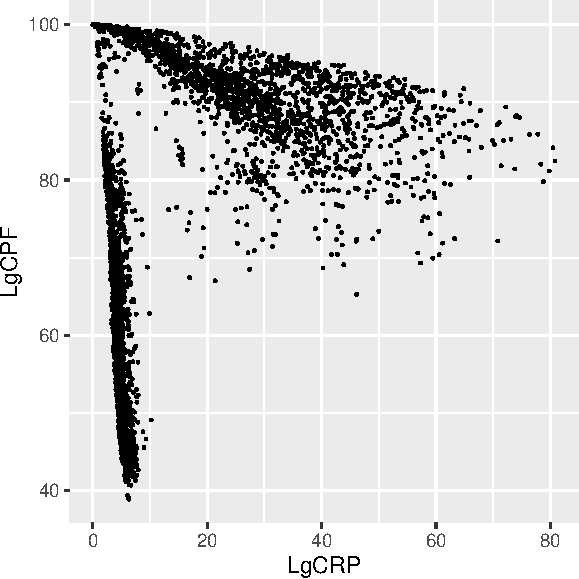
\includegraphics{rj_paper_files/figure-latex/comp-var-pairs-1} 

}

\caption[Scatterplots for numeric variable pairs with high difference among the magnitude of association measures]{Scatterplots for numeric variable pairs with high difference among the magnitude of association measures}\label{fig:comp-var-pairs}
\end{figure}
\end{Schunk}

Figure \ref{fig:comp-var-pairs} shows scatterplots for the three
variable pairs which are picked out from the multiple measures plot.
These pairs have a high magnitude difference for Pearson's and
Spearman's correlation.

\hypertarget{conditional-association-plot}{%
\subsection{Conditional Association
Plot}\label{conditional-association-plot}}

The function \texttt{pairwise\_2d\_plot} is used to display a matrix
layout of the conditional association for variable pairs in the dataset.
The display is produced by splitting the data by a partitioning variable
and calculating association for the variable pairs at each level of
partitioning variable using \texttt{calc\_assoc} function with
conditioning variable as the \texttt{by} argument. The calculated
association measures are then displayed using bars in a matrix plot. The
height and color of the bars are coded with the value of association
measure and the level of the partitioning variable respectively. These
displays are efficient for discovering variable pair with high
differences among the levels of partitioning variable in the data.

The measures of association calculated for every variable pair at every
level of conditioning serve as input to the \texttt{pairwise\_2d\_plot}
function. The \texttt{lassoc} and \texttt{uassoc} arguments look for a
tibble of association measures for the lower triangle and the upper
triangle of the matrix display respectively. The \texttt{uassoc}
argument is set to \texttt{NULL} by default and uses the same tibble
input as used by \texttt{lassoc} if not updated. The argument
\texttt{group\_var} is responsible for the grouping variable when
plotting the bars. The default value \texttt{by} uses the conditioning
variable and \texttt{measure\_type} is useful for displaying bars with
height and color of the bars coded by the value of association measure
and the type of association measure respectively.

Figure \ref{fig:cond-assoc} shows a conditional association plot for the
chronic kidney data. Each cell corresponding to a variable pair shows
two bars which correspond to the association measure (Pearson's
correlation for numeric pair, Kendall's tau-b for ordered pair and
canonical correlation coefficient for other combination of variables)
calculated at the levels of conditioning variable \texttt{htn}
i.e.~whether the patient suffers from hypertension or not. The dashed
line represents the overall association measure. The plot indicates that
there is a high difference in the measure (Pearson's correlation) value
for the variable pair sc and sod among the patients with and without
hypertension.

\begin{Schunk}
\begin{Sinput}
cond_assoc <- calc_assoc_by(df, by="htn")
pairwise_2d_plot(cond_assoc)
\end{Sinput}
\begin{figure}

{\centering 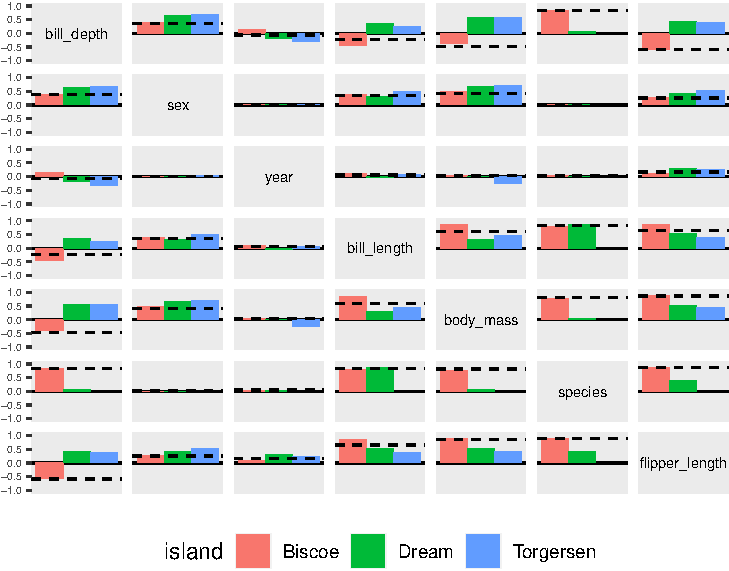
\includegraphics{rj_paper_files/figure-latex/cond-assoc-1} 

}

\caption[Conditional Association plot for chronic kidney data showing Pearson's correlation for numeric pairs, Kendall's tau-b for ordered pair and canonical correlation for nominal or mixed pairs]{Conditional Association plot for chronic kidney data showing Pearson's correlation for numeric pairs, Kendall's tau-b for ordered pair and canonical correlation for nominal or mixed pairs. The bars in each cell represent the value for asssociation measure colored by the conditioning variable `htn`. The dashed line in each cell represents overall value of the association measure.}\label{fig:cond-assoc}
\end{figure}
\end{Schunk}

Figure \ref{fig:high-diff} shows the scatterplot for the variable pair
sc and sod spllitted by the conditioning variable htn. The plot
indicates that there might be a stronger linear relationship among sc
and sod for the people having hypertension compared to patients without
hypertension. It is possible to filter out more variable pairs from the
conditional association plot having high difference for association
measure among the groups and further investigate these pairs.

\begin{Schunk}
\begin{figure}

{\centering 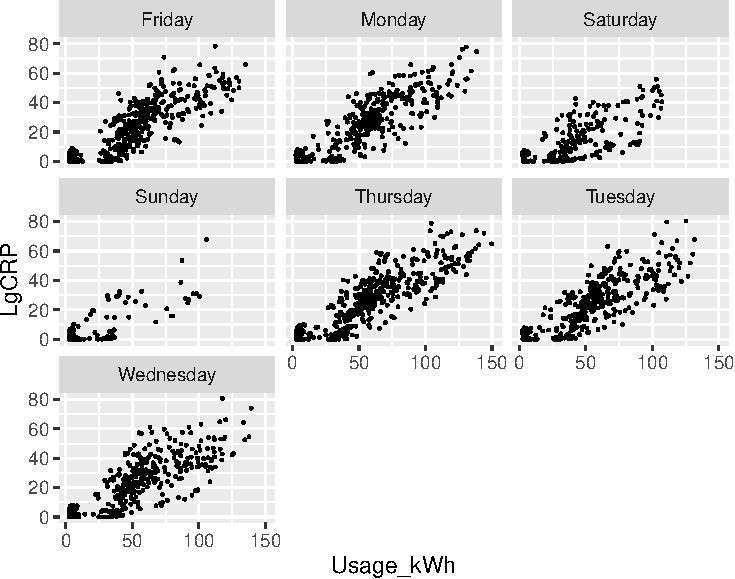
\includegraphics{rj_paper_files/figure-latex/high-diff-1} 

}

\caption[Scatterplot for variable pair sc and sod splitted by a conditioning variable htn]{Scatterplot for variable pair sc and sod splitted by a conditioning variable htn.}\label{fig:high-diff}
\end{figure}
\end{Schunk}

We also use linear layouts for displaying conditional association in the
package. The function \texttt{pairwise\_1d\_plot} is used for displaying
a linear layout of the conditional association for variable pairs in the
dataset. The association measures are calculated for every variable pair
at each level of partitioning variable using \texttt{calc\_assoc}
function with conditioning variable as the \texttt{by} argument.

The measures are then displayed using a dotplot where color of the dots
are coded by the level of the partitioning variable and the variable
pairs are ordered by absolute maximum value of association measure for
each of the pair of variable. These displays are also efficient for
discovering differences among the levels of partitioning variable in the
data. With the linear layouts it is easier to omit less relevant pairs
of variables by filtering the variables pairs having a higher value for
association measures than a threshold.

The measures of association calculated for every variable pair at every
level of conditioning serve as input to the \texttt{pairwise\_1d\_plot}
function. The \texttt{assoc} argument uses a tibble of association
measures calculated using \texttt{calc\_assoc} function with a
\texttt{by} variable. The argument \texttt{group\_var} is responsible
for the grouping variable when plotting the dots. The default value
\texttt{by} uses the conditioning variable and \texttt{measure\_type} is
useful for displaying dots with color of the dots coded by the type of
association measure. The \texttt{var\_order} argument is responsible for
the ordering of variable pairs in the display. If set to
\texttt{default} variable pairs are ordered alphabetically and are
ordered by absolute maximum value of association measure for every
variable pair when set to \texttt{max\_diff}.

Figure \ref{fig:linear-cond-assoc} shows a funnel-like linear display
for conditional association measures with all the variable pairs on the
y-axis, the value of association measure on x-axis and color of the
points representing the level of the grouping variable. The linear
layout becomes more useful over the matrix layout when the number of
variables and number of levels of grouping variable are high.

\begin{Schunk}
\begin{Sinput}
pairwise_1d_plot(cond_assoc)
\end{Sinput}
\begin{figure}

{\centering 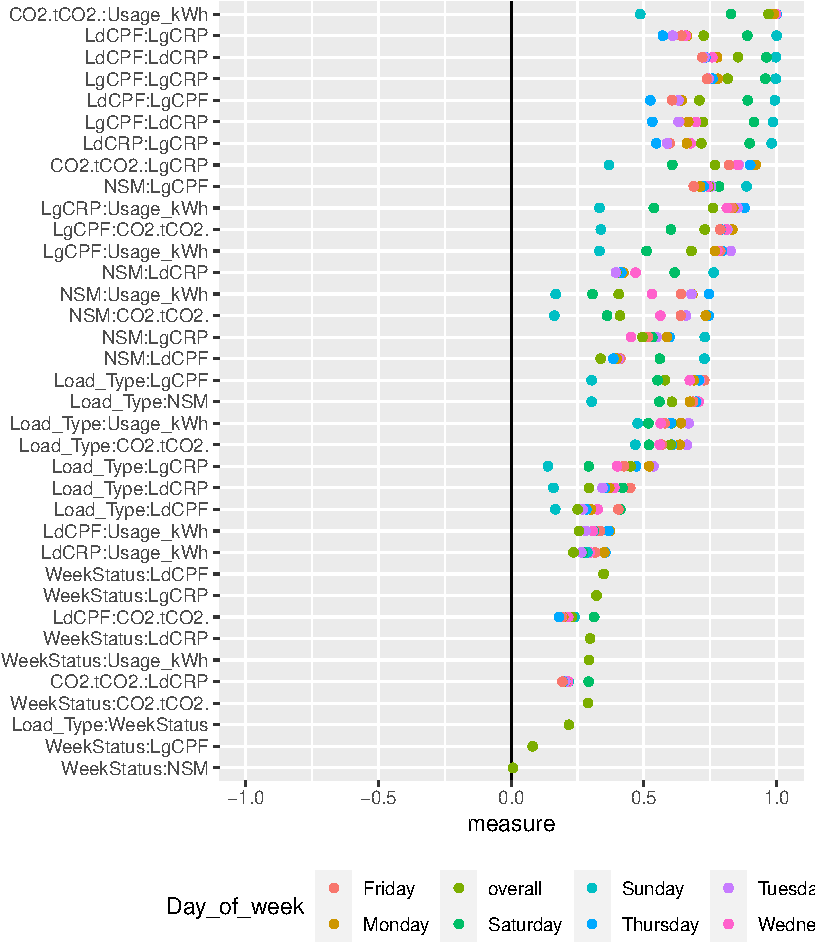
\includegraphics{rj_paper_files/figure-latex/linear-cond-assoc-1} 

}

\caption[Conditional Association plot using linear layout.The display has variable pairs on the Y-axis and the value of association measures on the X-axis]{Conditional Association plot using linear layout.The display has variable pairs on the Y-axis and the value of association measures on the X-axis. The points corresponding to every variable pair represents the value of association measure for different levels of the conditioning variable and the overall value of association measure.}\label{fig:linear-cond-assoc}
\end{figure}
\end{Schunk}

The \texttt{pairwise\_2d\_plot} function is also useful for comparing
various measures using the matrix layout. It plots multiple measures
among the variable pairs as bars, where each bar represents one measure
of association. Figure \ref{fig:compare-matrix} shows a matrix layout
comparing Pearson's and Spearman's correlation coefficient for the
numeric variable pairs in \texttt{penguins} data. The plot shows that
the value for both the correlation coefficients are very high for
\texttt{bill\_length} and \texttt{flipper\_length},
\texttt{bill\_length} and \texttt{body\_mass}, and
\texttt{flipper\_length} and \texttt{body\_mass} suggesting a strong
linear and montonic relationship among these variable pairs in the
dataset.

\begin{Schunk}
\begin{Sinput}
df_num <- select(df,where(is.numeric))
pearson <- calc_assoc(df_num)

spearman_assoc <- update_assoc(num_pair = "tbl_cor",
                               num_pair_argList= "spearman",
                               mixed_pair = "tbl_cancor",
                               other_pair = "tbl_nmi")
spearman <- calc_assoc(df_num, types=spearman_assoc)
compare <- rbind(pearson,spearman)
pairwise_2d_plot(compare, group_var = "measure_type")
\end{Sinput}
\begin{figure}

{\centering 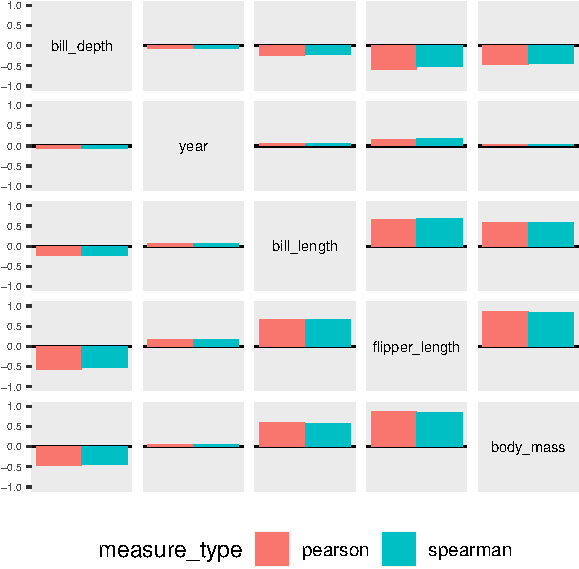
\includegraphics{rj_paper_files/figure-latex/compare-matrix-1} 

}

\caption[Matrix display comparing Pearson's and Spearman's correlation coefficient]{Matrix display comparing Pearson's and Spearman's correlation coefficient. All the variable pairs have similar values for both correlations.}\label{fig:compare-matrix}
\end{figure}
\end{Schunk}

\hypertarget{section-5-discussion}{%
\section{Section 5: Discussion}\label{section-5-discussion}}

We use multiple association measures in a single display for different
variable pairs which serves as a comparison tool while exploring
association in a dataset and assist in identifying unusual variable
pairs. These multiple measures can be displayed in a scatterplot matrix
similar to what \citet{tukey1985computer} proposed. They suggested that
scatterplot matrix of the scagnostics measures, which are measures
summarizing a scatterplot, can be used to identify unusual scatterplots
or variable pairs. \citet{wilkinson2005graph} used this idea with their
graph-theoretic scagnostic measures to highlight unusual scatterplots.
Similarly, \citet{kuhn2013applied} have used this idea in a predictive
modeling context. They have produced a scatterplot matrix of the
measures between the response and continuous predictors such as
Pearson's correlation coefficient, pseudo-\(R^2\) from the locally
weighted regression model, MIC and Spearman's rank correlation
coefficient to explore the predictor importance during feature selection
step. These displays show the importance of comparing multiple
association measures at once for different variable pairs.

\bibliography{RJreferences.bib}

\address{%
Amit Chinwan\\
Maynooth University\\%
Hamilton Institute\\ Maynooth, Ireland\\
%
%
%
\href{mailto:amit.chinwan.2019@mumail.ie}{\nolinkurl{amit.chinwan.2019@mumail.ie}}%
}

\address{%
Catherine Hurley\\
Maynooth University\\%
Department of Mathematics and Statistics\\ Maynooth, Ireland\\
%
%
%
\href{mailto:catherine.hurley@mu.ie}{\nolinkurl{catherine.hurley@mu.ie}}%
}
